% Material moved out of Supplementary Section S2 in v7 (not used by the main text).
% Compile as part of supplementary.tex (it uses its labels) or read as source.
% Tables are generated by experiments/build_paper_assets.py jpc-remediation.

\section{Tuning study (extended)}
These analyses concern the tunings themselves, not the anti-windup logic, and are not used by the conclusions of the main text. The two tunings below complete the test bed of the main text.
\begin{enumerate}
    \item \textbf{2-DOF AMIGO}: the AMIGO gains with setpoint weights $\beta = 0.5$, $\gamma = 0$ (Section~\ref{subsec:two_dof}), the use for which AMIGO is intended in servo tasks \cite{astrom2004revisiting}.
    \item \textbf{Optimal ITAE ($M_s^{\mathrm{FOPTD}} \le 1.6$)}: Nelder--Mead minimization of the ITAE of a $-2$~K step on the nonlinear plant and the benchmark valve, with the penalty $10^4\max(0, M_s - 1.6)^2$ and $M_s$ evaluated on the identified dead-time loop of Eq.~\eqref{eq:foptd}; the superscript records that the bound is imposed on the design model, not on the exact loop (Section~\ref{subsec:constraint_cost}). Evaluating $M_s$ on the delay-free Jacobian instead would return values close to one for almost any gain and silently disable the constraint. Because the simplex is local, it is started from a default guess and from every analytical tuning already inside the robust set (AMIGO, SIMC). The default start stops at a PI-like local optimum ($T_d = 0$, $\mathrm{ITAE} = 0.34$~K$\cdot$min$^2$); the analytical starts reach $0.20$--$0.21$~K$\cdot$min$^2$. The retained optimum has $M_s^{\mathrm{FOPTD}} = 1.60$: the constraint is active on the design model, and the derivative action is kept because it buys the phase margin that allows a higher proportional gain at the same $M_s$.
    \item \textbf{2-DOF Optimal ITAE}: the optimal gains with the setpoint weights fixed at $\beta = 0.5$, $\gamma = 0$. It is a 2-DOF \emph{variant}, not an optimized 2-DOF design.
\end{enumerate}

\subsection{Two-degree-of-freedom setpoint weighting}
\label{subsec:two_dof}
A 2-DOF structure weights the reference in the proportional and derivative paths \cite{astrom2006pid}. To avoid a bias from absolute temperatures when $\beta < 1$, the weights act on deviations from $y_{ss} = 396.65$~K:
\begin{equation}
    e_p = \beta\,\Delta y_{sp} - \Delta y_{pv}, \qquad e_i = y_{sp} - y_{pv}, \qquad e_d = \gamma\,\Delta y_{sp} - \Delta y_{pv},
    \label{eq:two_dof}
\end{equation}
with $\Delta y = y - y_{ss}$, so that $P_k = K_p e_{p,k}$, the integrator is driven by $e_{i,k}$ and the derivative by $e_{d,k}$; $\gamma = 0$ recovers derivative on the measurement. Because $\beta$ and $\gamma$ act only on the reference path, the loop transfer function $L(s) = G_p(s)C(s)$, and therefore $M_s$ and the load response, are those of the 1-DOF controller with the same gains.

\subsection{Sensitivity peak and margins}
\label{subsec:sensitivity_theory}
Robustness is quantified by the sensitivity peak \cite{astrom2006pid, skogestad2005multivariable}
\begin{equation}
    M_s = \sup_{\omega \ge 0} \left|\frac{1}{1 + G_p(j\omega)C(j\omega)}\right|,
    \label{eq:sensitivity_func}
\end{equation}
evaluated with the exact delay $e^{-j\omega\theta}$ and $C(s) = K_p\,(1 + 1/(T_i s) + T_d s/(\tau_f s + 1))$. The bound $M_s \le 1.6$ guarantees a gain margin of at least $2.67$ and a phase margin of at least $36.4^\circ$ \cite{garpinger2014performance, padula2011tuning}. The FOPTD and the true plant agree at low frequency but diverge above the identification bandwidth: the delay adds phase lag without bound, whereas the phase of the relative-degree-two $G_{\text{true}}$ saturates. The FOPTD therefore overestimates the high-frequency lag, which makes $M_s$ conservative for loops whose peak lies at high frequency, while near crossover the comparison can go either way. Section~\ref{subsec:margins} evaluates both loops.

\subsection{Nominal step with the setpoint-weighted variants}
\begin{table*}[t]
\centering
\footnotesize
\caption{Nominal servo benchmark ($-2$~K setpoint step, noise-free) on the non-linear CSTR. FOPTD: $K=-0.1852$~K/(L/min), $\tau=0.6427$~min, $\theta=0.0935$~min. $M_s$ is evaluated on the dead-time FOPTD loop; TV includes the initial valve move from $\bar q_j$.}
\label{tab:classical_benchmark}
\resizebox{\ifdim\width>\textwidth\textwidth\else\width\fi}{!}{%
\begin{tabular}{lcccccccccc}
\toprule
Method & \(K_p\) & \(T_i\text{ (min)}\) & \(T_d\text{ (min)}\) & \(\beta\) & IAE & ITAE (K$\cdot$min$^2$) & TV (L/min) & \(M_p\text{ (\%)}\) & \(t_s\text{ (min)}\) & \(M_s\) \\
\midrule
Ziegler-Nichols & -44.56 & 0.187 & 0.047 & 1.0 & 0.940 & 0.316 & 81.9 & 22.6 & 1.38 & 4.14 \\
Cohen-Coon & -50.86 & 0.217 & 0.033 & 1.0 & 1.017 & 0.388 & 104.0 & 31.0 & 1.40 & 4.54 \\
Tyreus-Luyben & -28.10 & 0.779 & 0.056 & 1.0 & 0.917 & 0.336 & 48.8 & 0.0 & 1.64 & 2.32 \\
AMIGO & -17.79 & 0.327 & 0.045 & 1.0 & 0.925 & 0.308 & 40.4 & 9.7 & 1.44 & 1.45 \\
2-DOF AMIGO & -17.79 & 0.327 & 0.045 & 0.5 & 0.962 & 0.312 & 29.3 & 5.3 & 1.48 & 1.45 \\
Skogestad SIMC & -7.03 & 0.643 & 0.031 & 1.0 & 1.288 & 0.629 & 15.7 & 0.0 & 1.96 & 1.13 \\
Optimal ITAE ($M_s \leq 1.6$) & -23.55 & 0.465 & 0.032 & 1.0 & 0.827 & 0.204 & 48.6 & 2.2 & 0.94 & 1.60 \\
2-DOF Optimal ITAE & -23.55 & 0.465 & 0.032 & 0.5 & 1.084 & 0.424 & 25.0 & 0.0 & 1.62 & 1.60 \\
\bottomrule
\end{tabular}%
}
\end{table*}


With the directional rule of Eq.~\eqref{eq:clamping_antiwindup}, every tuning tracks the step. ZN and CC reach competitive errors ($\mathrm{IAE} = 0.940$ and $1.017$~K$\cdot$min) but with $M_s = 4.14$ and $4.54$, overshoots of $22.6\%$ and $31.0\%$ and $81.9$ and $104.0$~L/min of valve travel. Tyreus--Luyben gives $\mathrm{IAE} = 0.917$~K$\cdot$min without overshoot despite $M_s = 2.32$, and AMIGO ($M_s = 1.45$) gives $0.925$~K$\cdot$min with $9.7\%$ overshoot. Setpoint weighting reduces the AMIGO overshoot to $5.3\%$ and its travel from $40.4$ to $29.3$~L/min for a small increase in error ($0.962$~K$\cdot$min). SIMC ($M_s = 1.13$) is the most conservative tuning ($\mathrm{IAE} = 1.288$~K$\cdot$min, $\mathrm{TV} = 15.7$~L/min). Optimal ITAE, with its design-model constraint active ($M_s^{\mathrm{FOPTD}} = 1.60$), is the fastest loop of the benchmark ($\mathrm{IAE} = 0.827$~K$\cdot$min, $\mathrm{ITAE} = 0.204$~K$\cdot$min$^2$, settling in $0.94$~min with $2.2\%$ overshoot); its 2-DOF variant removes the overshoot and roughly halves the travel ($25.0$~L/min) at $\mathrm{IAE} = 1.084$~K$\cdot$min.

\subsection{Design-model versus plant robustness}
\label{subsec:margins}
Figure~\ref{fig:sensitivity_magnitude} shows $|S(j\omega)|$ on the FOPTD, and Table~\ref{tab:loop_margins} compares $M_s$ and the phase margin on the FOPTD and on the exact linearization of the plant with the half-sample hold delay $\Delta t/2$.

\begin{figure}[t]
    \centering
    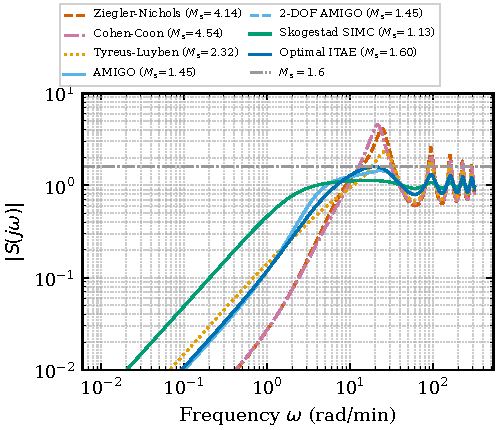
\includegraphics[width=0.55\textwidth]{figures/fig_sensitivity_magnitude.pdf}
    \caption{Sensitivity magnitude $|S(j\omega)|$ on the identified dead-time FOPTD model. The 2-DOF variants share the loop of their 1-DOF counterparts.}
    \label{fig:sensitivity_magnitude}
\end{figure}

\begin{table*}[t]
\centering
\footnotesize
\caption{Sensitivity peak and phase margin of each PID loop on the identified FOPTD design model and on the exact Jacobian linearization of the CSTR at $\mathbf{x}_{ss}$ with the half-sample zero-order-hold delay $\Delta t/2 = 0.01$~min. Valve saturation and slew-rate limits are not part of either linear loop.}
\label{tab:loop_margins}
\resizebox{\ifdim\width>\textwidth\textwidth\else\width\fi}{!}{%
\begin{tabular}{lcccc}
\toprule
Method & \(M_s\) (FOPTD) & PM (FOPTD, \(^\circ\)) & \(M_s\) (lin.) & PM (lin., \(^\circ\)) \\
\midrule
Ziegler-Nichols & 4.14 & 36.6 & 1.57 & 38.4 \\
Cohen-Coon & 4.54 & 25.3 & 1.75 & 35.1 \\
Tyreus-Luyben & 2.32 & 72.3 & 1.15 & 71.1 \\
AMIGO & 1.45 & 59.3 & 1.26 & 53.9 \\
Skogestad SIMC & 1.13 & 81.7 & 1.11 & 78.7 \\
Optimal ITAE ($M_s^{\mathrm{FOPTD}} \leq 1.6$) & 1.60 & 61.1 & 1.31 & 57.1 \\
\bottomrule
\end{tabular}%
}
\end{table*}


The sensitivity peak on the linearized plant is lower than on the FOPTD for every tuning, and strongly so for the high-gain rules (ZN: $4.14 \rightarrow 1.57$, CC: $4.54 \rightarrow 1.75$, TL: $2.32 \rightarrow 1.15$). Their peaks lie at high frequency, where the FOPTD delay keeps adding phase lag that the relative-degree-two plant of Eq.~\eqref{eq:g_true_exact} does not have; together with the rate limit, which clips the initial proportional kick into a bounded ramp, this explains why ZN and CC do not oscillate on the noise-free step. The phase margin, set near crossover, behaves differently: for the moderate-bandwidth designs the FOPTD is slightly optimistic (AMIGO: $59.3^\circ$ versus $53.9^\circ$, Optimal ITAE: $61.1^\circ$ versus $57.1^\circ$, SIMC: $81.7^\circ$ versus $78.7^\circ$), whereas for ZN and CC it is pessimistic ($36.6^\circ$ versus $38.4^\circ$ and $25.3^\circ$ versus $35.1^\circ$). The $M_s \le 1.6$ constraint imposed on the FOPTD is thus a conservative proxy for the peak sensitivity of the real loop (Section~\ref{subsec:constraint_cost} measures what that conservatism costs), but the designer should allow for a loss of up to $5.4^\circ$ of phase margin at crossover. Neither linear loop contains the rate limit, which adds an amplitude-dependent phase lag during large moves; the table describes small-signal behaviour.

\begin{table*}[t]
\centering
\footnotesize
\caption{Plant-exact robustness of the six feedback loops on the Jacobian linearization at $\mathbf{x}_{ss}$ with the half-sample zero-order-hold delay, and the high-frequency controller gain that maps measurement noise into valve movement.}
\label{tab:exact_robustness}
\resizebox{\ifdim\width>\textwidth\textwidth\else\width\fi}{!}{%
\begin{tabular}{lccccc}
\toprule
Method & \(M_s\) (FOPTD) & \(\|S\|_\infty\) (lin.) & \(\|T\|_\infty\) (lin.) & \(\|CS\|_\infty\) (L/min/K) & \(K_{\mathrm{hf}}=|K_p|(1+N)\) (L/min/K) \\
\midrule
Ziegler-Nichols & 4.14 & 1.57 & 1.66 & 490.1 & 490.2 \\
Cohen-Coon & 4.54 & 1.75 & 1.72 & 559.2 & 559.5 \\
Tyreus-Luyben & 2.32 & 1.15 & 1.00 & 309.0 & 309.1 \\
AMIGO & 1.45 & 1.26 & 1.22 & 195.6 & 195.7 \\
Skogestad SIMC & 1.13 & 1.11 & 1.00 & 77.3 & 77.4 \\
Optimal ITAE ($M_s^{\mathrm{FOPTD}} \leq 1.6$) & 1.60 & 1.31 & 1.11 & 258.9 & 259.0 \\
\bottomrule
\end{tabular}%
}
\end{table*}


The sensitivity peak does not explain the noise behaviour of the empirical rules, because on the exact linearization their peaks are only $\|S\|_\infty = 1.57$ (ZN) and $1.75$ (CC); the values of $4.14$ and $4.54$ on the design model largely reflect the apparent delay of the FOPTD. What does distinguish the loops is the gain from measurement noise to the valve command, $CS = C/(1+L)$ (Table~\ref{tab:exact_robustness}). At high frequency $S \to 1$ and $CS \to C$, so $\|CS\|_\infty$ is attained on the plateau of the filtered PID, $K_{\mathrm{hf}} = |K_p|(1+N)$, and equals it to within $0.3$~L/min/K for all six loops: $490.1$ (ZN), $559.2$ (CC), $309.0$ (TL), $195.6$ (AMIGO), $258.9$ (Optimal ITAE) and $77.3$ (SIMC) L/min/K. ZN and CC therefore convert measurement noise into valve movement with $6$ to $7$ times the gain of SIMC, even though their loops are not close to instability.

\subsection{Cost of imposing the sensitivity bound on the design model}
\label{subsec:constraint_cost}
The Optimal ITAE tuning bounds $M_s$ on the identified dead-time model, whose apparent delay overstates the high-frequency lag; on the exact linearization the same gains have $M_s^{\mathrm{lin}} = 1.31$ and a phase margin of $57.1^\circ$ (Table~\ref{tab:constraint_cost}). To measure what the proxy costs, the optimization was repeated with $M_s^{\mathrm{lin}} \le 1.6$ imposed on the exact Jacobian loop with the half-sample zero-order hold, with the same objective, valve and multi-start (started from the default guess and from every analytical tuning inside the exact robust set, then restarted once from the winner).

\begin{table*}[t]
\centering
\footnotesize
\caption{Cost of the design-model constraint. Each tuning minimizes the ITAE of the $-2$~K step ($6$~min) subject to $M_s \le 1.6$ evaluated on the dead-time FOPTD ($M_s^{\mathrm{FOPTD}}$) or on the exact Jacobian loop with the half-sample zero-order hold ($M_s^{\mathrm{lin}}$); ``joint'' rows optimize $(K_p, T_i, T_d, \beta, \gamma)$ together, the 2-DOF row with $\beta = 0.5$ is the fixed-weight variant ($\beta = 0.5$, $\gamma = 0$) of Fig.~\ref{fig:classical_benchmark}. ITAE in K$\cdot$min$^2$, IAE in K$\cdot$min, TV in L/min, $K_{\mathrm{hf}}$ in (L/min)/K, PM at the highest gain crossover.}
\label{tab:constraint_cost}
\resizebox{\ifdim\width>\textwidth\textwidth\else\width\fi}{!}{%
\begin{tabular}{lccccccccccccccc}
\toprule
Tuning & \(K_p\) & \(T_i\) (min) & \(T_d\) (min) & \(\beta\) & \(\gamma\) & \(M_s^{\mathrm{FOPTD}}\) & \(M_s^{\mathrm{lin}}\) & PM$^{\mathrm{lin}}$ ($^\circ$) & \(K_{\mathrm{hf}}\) & IAE & ITAE & \(M_p\) (\%) & TV & ITAE $-5$ K & ITAE $+5$ K \\
\midrule
Optimal ITAE ($M_s^{\mathrm{FOPTD}} \leq 1.6$) & -23.55 & 0.465 & 0.032 & 1.00 & 0.00 & 1.60 & 1.31 & 57.1 & 259 & 0.827 & 0.204 & 2.2 & 48.6 & 1.292 & 1.200 \\
2-DOF Optimal ITAE & -23.55 & 0.465 & 0.032 & 0.50 & 0.00 & 1.60 & 1.31 & 57.1 & 259 & 1.084 & 0.424 & 0.0 & 25.0 & 1.756 & 1.564 \\
Joint 2-DOF ITAE ($M_s^{\mathrm{FOPTD}} \leq 1.6$) & -23.55 & 0.464 & 0.032 & 1.00 & 0.00 & 1.60 & 1.31 & 57.1 & 259 & 0.827 & 0.204 & 2.2 & 48.6 & 1.289 & 1.197 \\
Optimal ITAE ($M_s^{\mathrm{lin}} \leq 1.6$) & -41.41 & 0.597 & 0.093 & 1.00 & 0.00 & 13.86 & 1.20 & 75.5 & 456 & 0.799 & 0.181 & 0.7 & 59.6 & 1.322 & 1.239 \\
Joint 2-DOF ITAE ($M_s^{\mathrm{lin}} \leq 1.6$) & -46.23 & 0.558 & 0.099 & 0.98 & 0.09 & 12.95 & 1.24 & 74.4 & 508 & 0.799 & 0.181 & 0.8 & 60.7 & 1.307 & 1.257 \\
\bottomrule
\end{tabular}%
}
\end{table*}


The exact-loop optimum is interior: it stops at $M_s^{\mathrm{lin}} = 1.20$ ($\mathrm{PM} = 75.5^\circ$), so the exact bound is not active and it is the valve, not robustness, that caps the speed of the loop. Relaxing the design model to the exact loop lowers the design ITAE from $0.204$ to $0.181$~K$\cdot$min$^2$ ($-11.3\%$) and the IAE from $0.827$ to $0.799$~K$\cdot$min ($-3.4\%$), with overshoot $0.7\%$, at the price of a $1.76$ times higher proportional gain: the high-frequency gain rises from $259$ to $456$~L/min/K ($+76\%$) and the valve travel from $48.6$ to $59.6$~L/min ($+22.6\%$). The gain does not carry over outside the design step: the ITAE on the $-5$ and $+5$~K steps is $2.3\%$ and $3.3\%$ \emph{higher} than that of the FOPTD-bounded tuning (last two columns of Table~\ref{tab:constraint_cost}). The 11\% ITAE of the exact-loop optimum is therefore an in-sample gain with no counterpart outside the design step, and it is paid for in noise gain: the FOPTD-bounded tuning has $43\%$ lower high-frequency gain ($259$ against $456$~L/min/K). The phrase ``fastest robust PID'' is not used for either tuning, because the speed of the first is capped by the proxy and that of the second by the rate limit.

\paragraph{Model error.} The margin of the exact-loop optimum is also more exposed to model error (Table~\ref{tab:model_error}). The test is like-for-like: the same exact plant and the same $18$ perturbations for every tuning (loop gain and all plant time constants, $\tau$ included, scaled by $0.8$, $1$ and $1.2$, and an extra delay of $0$ or $0.2\,\theta_{\mathrm{FOPTD}}$), with the stability of every corner decided from the closed-loop polynomial and $M_s$ taken over the stable corners only. No tuning has an unstable corner. The worst $M_s$ is $1.63$ for the FOPTD-bounded optimum ($1.31$ nominal), $2.06$ for the exact-loop optimum ($1.20$ nominal), $2.84$ and $3.42$ for ZN and CC, $1.42$ for TL, $1.59$ for AMIGO and $1.20$ for SIMC: its peak rises by $72\%$ over the nominal value against $24\%$ for the FOPTD-bounded one, but it stays stable at every corner and better than ZN and CC. Deadband (Section~\ref{subsec:ablation}) was simulated for the anti-windup policies and not for $M_s$; stiction was not simulated.

\begin{table*}[t]
\centering
\footnotesize
\caption{Sensitivity peak under model error: on the FOPTD, the largest $M_s$ over the $27$ corners of $K$, $\tau$, $\theta$ scaled by $0.8$, $1$, $1.2$; on the exact loop, the largest $M_s$ with the loop gain scaled by $0.8$ or $1.2$ and an extra delay of $0.2\,\theta_{\mathrm{FOPTD}}$. Deadband and stiction are not modelled.}
\label{tab:model_error}
\resizebox{\ifdim\width>\textwidth\textwidth\else\width\fi}{!}{%
\begin{tabular}{lcccc}
\toprule
Tuning & \(M_s^{\mathrm{FOPTD}}\) nominal & worst of $27$ corners & \(M_s^{\mathrm{lin}}\) nominal & worst ($K\pm20\%$, $+0.2\theta$) \\
\midrule
Optimal ITAE ($M_s^{\mathrm{FOPTD}} \leq 1.6$) & 1.60 & 2.74 & 1.31 & 1.56 \\
Optimal ITAE ($M_s^{\mathrm{lin}} \leq 1.6$) & 13.86 & 151.77 & 1.20 & 1.60 \\
AMIGO & 1.45 & 2.02 & 1.26 & 1.44 \\
Skogestad SIMC & 1.13 & 1.25 & 1.11 & 1.18 \\
\bottomrule
\end{tabular}%
}
\end{table*}


\paragraph{Moved to the repository.} The out-of-sample ITAE of every tuning, the tracking-error versus valve-travel locus of SIMC (with its figure and table) and the joint optimization of gains and setpoint weights are not used by the main text; they are in \texttt{papers/01\_journal\_of\_process\_control/repository/S2\_tuning\_extended.tex} of the code repository, generated by the same scripts.



\subsection{Joint optimization of gains and setpoint weights}
Optimizing the setpoint weights jointly with the gains returns the 1-DOF controller. Under the FOPTD bound the optimum has $\beta = 1.00$ and $\gamma = 0.00$ with the same ITAE ($0.204$); under the exact bound $\beta = 0.98$ and $\gamma = 0.09$ with the same ITAE ($0.181$) and a $12\%$ higher proportional gain. Setpoint weighting does not help a tracking objective that has no cost on the valve; the fixed weight $\beta = 0.5$ of the 2-DOF variant is a deliberate trade of $+31.1\%$ IAE for $-48.6\%$ valve travel and no overshoot, not an optimum, and it is called a variant, not ``optimal'', in the remainder of the paper.


\subsection{Out-of-sample setpoint steps}
\label{subsec:oos}
The Optimal ITAE gains were fitted on the $-2$~K step, so their advantage in Table~\ref{tab:classical_benchmark} is in-sample. Table~\ref{tab:out_of_sample} evaluates every tuning on steps of $-5$, $-1$, $+1$, $+2$ and $+5$~K with the same valve, anti-windup and horizon ($10$~min; the optimizer used $6$~min).

\begin{table*}[t]
\centering
\footnotesize
\caption{ITAE (K$\cdot$min$^2$) of every tuning on setpoint steps of different size and sign. The Optimal ITAE gains were fitted on the $-2$~K step only (in-sample column); all other columns are out-of-sample. Same valve, directional anti-windup and $10$~min horizon.}
\label{tab:out_of_sample}
\resizebox{\ifdim\width>\textwidth\textwidth\else\width\fi}{!}{%
\begin{tabular}{lcccccc}
\toprule
Method & -5 K & -2 K & -1 K & +1 K & +2 K & +5 K \\
\midrule
Ziegler-Nichols & 1.413 & 0.316 & 0.084 & 0.105 & 0.345 & 1.985 \\
Cohen-Coon & 1.571 & 0.388 & 0.111 & 0.131 & 0.465 & 3.373 \\
Tyreus-Luyben & 1.876 & 0.336 & 0.092 & 0.091 & 0.327 & 1.716 \\
AMIGO & 1.389 & 0.308 & 0.122 & 0.108 & 0.250 & 0.969 \\
2-DOF AMIGO & 1.605 & 0.312 & 0.118 & 0.105 & 0.260 & 1.136 \\
Skogestad SIMC & 2.961 & 0.629 & 0.229 & 0.204 & 0.499 & 1.890 \\
Optimal ITAE ($M_s \leq 1.6$) & 1.292 & 0.204 & 0.065 & 0.063 & 0.192 & 1.200 \\
2-DOF Optimal ITAE & 1.756 & 0.424 & 0.154 & 0.153 & 0.414 & 1.564 \\
Rank of Optimal ITAE (1 = best) & 1 & 1 & 1 & 1 & 1 & 3 \\
\bottomrule
\end{tabular}%
}
\end{table*}


The optimum generalizes to steps of both signs up to $5$~K in the cooling direction and $2$~K in the heating direction: among the eight benchmark tunings it has the lowest ITAE at $-5$ ($1.292$), $-1$ ($0.065$), $+1$ ($0.063$) and $+2$~K ($0.192$). At $+5$~K it ranks third ($1.200$), behind AMIGO ($0.969$) and 2-DOF AMIGO ($1.136$), so the in-sample optimum is not uniformly optimal for the largest heating step. The tunings that were re-optimized in Section~\ref{subsec:constraint_cost} do not change the picture: the exact-loop optimum wins in-sample ($0.181$) and at $+1$~K ($0.062$) but loses to the FOPTD-bounded one at $-5$, $-1$, $+2$ and $+5$~K, and the jointly optimized 2-DOF designs coincide with their 1-DOF counterparts to within $0.02$~K$\cdot$min$^2$.

\subsection{Tracking error versus valve travel}
\label{subsec:pareto_results}
The trade-off between tracking accuracy and actuator wear was mapped by sweeping the SIMC closed-loop time constant over $\tau_c \in [0.015, 2.5]$~min ($45$ logarithmically spaced points) and by minimizing $\lambda\,\mathrm{IAE}/\mathrm{IAE}_0 + (1 - \lambda)\,\mathrm{TV}/\mathrm{TV}_0$ for $\lambda \in [0.05, 0.95]$ (Fig.~\ref{fig:pareto_iae_tv}, Table~\ref{tab:pareto_tradeoff}).

\begin{figure*}[t]
    \centering
    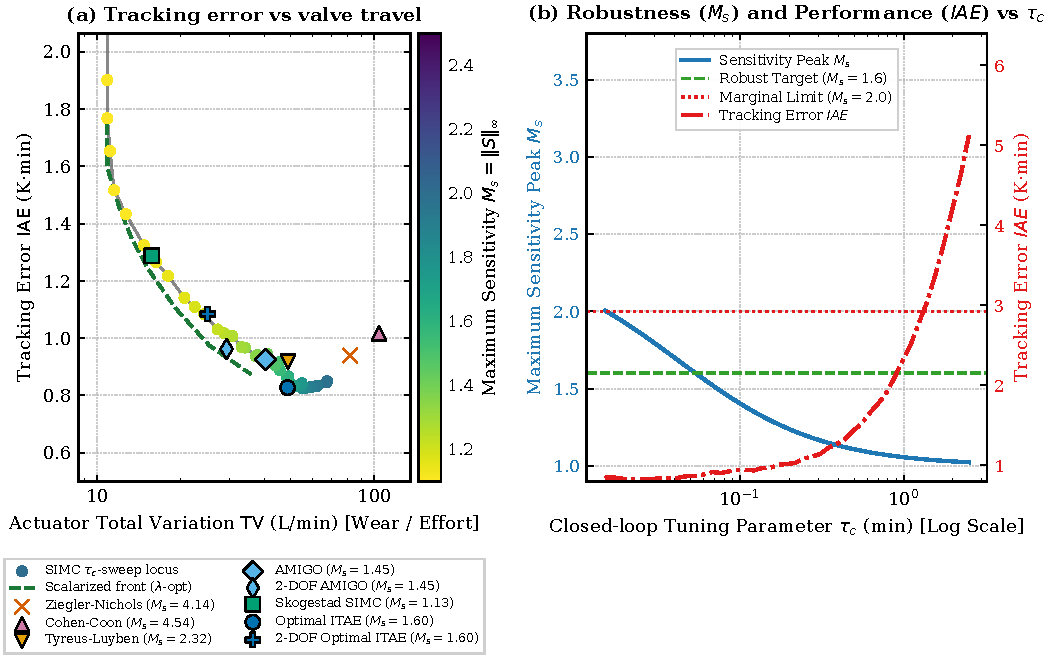
\includegraphics[width=0.92\textwidth]{figures/fig4_pareto_iae_tv.pdf}
    \caption{(a) SIMC $\tau_c$-sweep locus (colour: $M_s$), scalarized optimal front ($\lambda$-opt) and the discrete tunings in the $(\mathrm{TV}, \mathrm{IAE})$ plane (logarithmic TV axis); (b) $M_s$ and IAE as functions of $\tau_c$.}
    \label{fig:pareto_iae_tv}
\end{figure*}

\begin{table*}[t]
\centering
\footnotesize
\caption{Trade-off along the SIMC $\tau_c$ locus and for the discrete rules: robustness ($M_s$), tracking error and actuator effort (TV); the locus is a one-parameter family, not a Pareto frontier.}
\label{tab:pareto_tradeoff}
\resizebox{\ifdim\width>\textwidth\textwidth\else\width\fi}{!}{%
\begin{tabular}{lccccccc}
\toprule
Strategy & $K_{p}$ & $T_{i}$ (min) & $T_{d}$ (min) & $M_{s}$ & IAE (K$\cdot$min) & TV (L/min) & $M_{p}$ (\%) \\
\midrule
SIMC ($\tau_c=0.03$) & -28.08 & 0.49 & 0.03 & 1.79 & 0.83 & 54.2 & 0.3 \\
SIMC ($\tau_c=0.10$) & -18.28 & 0.64 & 0.03 & 1.41 & 0.95 & 41.0 & 0.0 \\
SIMC ($\tau_c=0.24$) & -10.27 & 0.64 & 0.03 & 1.20 & 1.08 & 24.3 & 0.0 \\
SIMC ($\tau_c=0.39$) & -7.19 & 0.64 & 0.03 & 1.13 & 1.27 & 16.3 & 0.0 \\
SIMC ($\tau_c=0.78$) & -3.97 & 0.64 & 0.03 & 1.07 & 1.90 & 10.9 & 0.0 \\
SIMC ($\tau_c=1.57$) & -2.09 & 0.64 & 0.03 & 1.04 & 3.40 & 10.9 & 0.0 \\
Ziegler-Nichols & -44.56 & 0.19 & 0.05 & 4.14 & 0.94 & 81.9 & 22.6 \\
Cohen-Coon & -50.86 & 0.22 & 0.03 & 4.54 & 1.02 & 104.0 & 31.0 \\
Tyreus-Luyben & -28.10 & 0.78 & 0.06 & 2.32 & 0.92 & 48.8 & 0.0 \\
AMIGO & -17.79 & 0.33 & 0.04 & 1.45 & 0.93 & 40.4 & 9.7 \\
2-DOF AMIGO & -17.79 & 0.33 & 0.04 & 1.45 & 0.96 & 29.3 & 5.3 \\
Skogestad SIMC & -7.03 & 0.64 & 0.03 & 1.13 & 1.29 & 15.7 & 0.0 \\
Optimal ITAE ($M_s^{\mathrm{FOPTD}} \leq 1.6$) & -23.55 & 0.47 & 0.03 & 1.60 & 0.83 & 48.6 & 2.2 \\
2-DOF Optimal ITAE & -23.55 & 0.47 & 0.03 & 1.60 & 1.08 & 25.0 & 0.0 \\
\bottomrule
\end{tabular}%
}
\end{table*}


Along the SIMC locus the error decreases monotonically as $\tau_c$ shrinks ($1.90$, $1.27$, $1.08$, $0.95$ and $0.83$~K$\cdot$min for $\tau_c = 0.78$, $0.39$, $0.24$, $0.10$ and $0.03$~min) while $M_s$ rises from $1.07$ to $1.79$ and the travel from $10.9$ to $54.2$~L/min: speed is bought with robustness, and with a correct anti-windup the rate limit creates no interior optimum. For $\tau_c \ge 0.78$~min the travel reaches its floor of $10.9$~L/min, the net change of steady-state coolant flow required by the new setpoint. The scalarized front lies slightly below the SIMC locus, so a free PID improves on SIMC by a small margin at equal travel. SIMC, 2-DOF AMIGO and 2-DOF Optimal ITAE lie close to the front; AMIGO, TL and Optimal ITAE sit on its high-gain branch; ZN and CC are dominated, with more error and more travel than Optimal ITAE at $2.6$ to $2.8$ times its design $M_s$.

